\documentclass[14pt]{extarticle}
\usepackage{graphicx}
\usepackage{amsmath}
\usepackage{xcolor}





\begin{document}

\title{Organizzazione e Gestione per lo startup Aziendale}
\author{Alessandro Savioli}
\date{Febbraio 2025}

\maketitle

\tableofcontents

\newpage

\section{Lezione 1}

\section{Lezione 2}

\section{Lezione 3}
\subsection{La Struttura Organizzativa}

\textbf{Organizzare} significa ordinare un sistema di parti dipendenti tra loro,
definendo per ognuna uno specifico ruolo all'interno del sistema stesso.

Per fare ciò, serve trovare una \textcolor{red}{Struttura Organizzativa}, in cui
possiamo trovare:
\begin{enumerate}
    \item Un insieme di relazioni tra le persone interne all'azienda;
    \item Una distribuzione delle Autorità e delle Responsabilità;
    \item Un insieme di processi con i quali l'azienda si costituisce.
\end{enumerate}
Questa struttura non può essere formulata partendo da un modello ideale ed
astratto, bensì deve essere \textbf{adattata} alla realtà nella quale l'azienda
opera.

Una struttura organizzativa è composta da elementi:
\begin{itemize}
    \item \textbf{Hardware (o di struttura)} meccanismo attraverso il quale
    vengono affidate delle funzioni a tutte le parti del sistema;
    \item \textbf{Software (o decisionali)} che stabilisce scopo, finalità e \\
    obiettivi dell'organizzazione e ne elabora le norme e le relazioni delle
    parti.  
\end{itemize}
Inoltre, una struttura organizzativa può essere di tipo:

\begin{itemize}
    \item \textbf{Formale}, dove la divisione in mansioni e la loro integrazione
    è esplicitamente riconosciuta e può essere rappresentata tramite gli
    \textbf{organigrammi};
    \item \textbf{Informale}, che fa riferimento a rapporti spontanei e a
    fattori di influenza e potere. 
\end{itemize}

\subsection{Gli Organigrammi}

Gli organigrammi sono delle rappresentazioni grafiche globali, di facile
comprensione, della struttura organizzativa formale dell'impresa.

Il loro scopo è quello di evidenziare gli aspetti fondamentali del funzionamento
dell'organizzazione, le posizioni strutturali ed i collegamenti tra le diverse
funzioni aziendali.
\begin{center}
    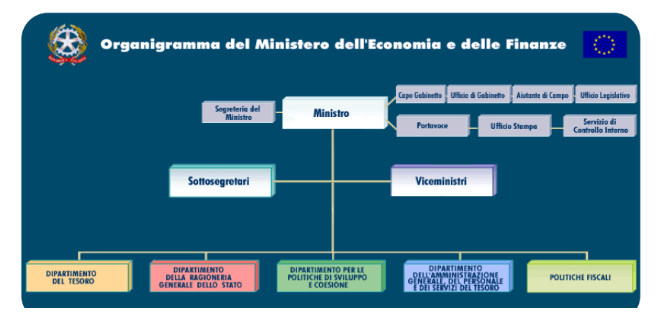
\includegraphics[scale = 0.80]{images/Esempio_Organigramma}
    Esempio di un organigramma 
\end{center}
Questo tipo di rappresentazione grafica ha però dei difetti, in quanto si fa
difficoltà a capire l'importanza delle posizioni rappresentate, non si hanno
informazioni sui rapporti non gerarchici e non si capisce in che ambiente opera
l'azienda.

\subsection{I vari Tipi di Struttura Organizzativa}
\subsubsection{Il modello Gerarchico (Struttura Monofunzionale)}

\begin{center}
    \textcolor{red!50}{CARATTERISTICHE}
\end{center}


\begin{itemize}
    \item \textbf{Principio di gerarchia}, secondo il quale \\ autorità,
    responsabilità e le competenze sono massime al vertice dell'organizzazione;
    \item \textbf{Principio di delega}, secondo il quale le funzioni vengono
    delegate verso il basso;
    \item \textbf{Principio di eccezione}, secondo il quale, in caso di
    difficoltà impreviste il problema deve tornare al vertice per essere
    risolto;
    \item \textbf{Principio dell'unità di direzione}, secondo il quale ciascuno
    deve aver ben chiaro da chi prendere ordini e a chi rivolgersi quando non
    sia in grado di decidere da solo.  
\end{itemize}

\begin{center}
    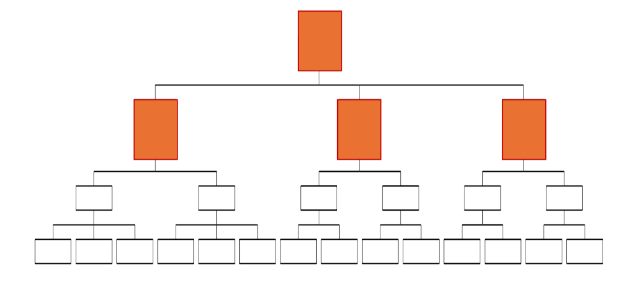
\includegraphics[scale = 0.80]{images/modello_gerarchico}
    Esempio di modello gerarchico
\end{center}

\newpage

\subsubsection{Il modello Gerarchico Funzionale (Struttura Gerarchico Funzionale)}

\begin{center}
    \textcolor{red!50}{CARATTERISTICHE}
\end{center}

Questo modello presenta attività raggruppate in base ad una funzione comune ed
esalta il \textbf{principio della specializzazione} delle singole aree.

Continua a seguire il \textbf{Principio di gerarchia} ed il \textbf{Principio di
eccezione} dal modello precedente.

\begin{center}
    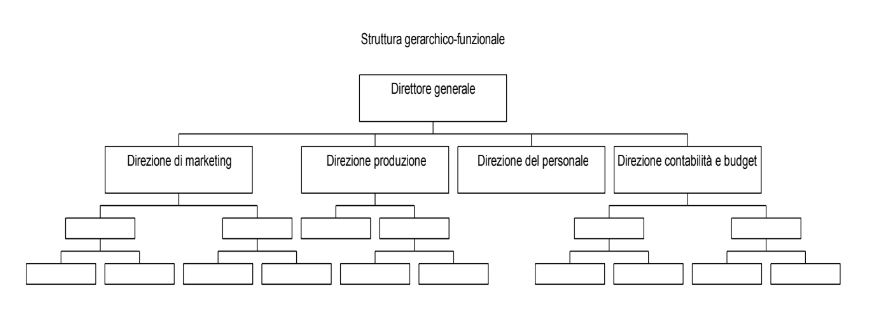
\includegraphics[scale = 0.64]{images/modello_gerarchico_funzionale}
    Esempio di modello gerarchico funzionale
\end{center}
Nella struttura gerarchico funzionale esistono tre livelli organizzativi
fondamentali:

\begin{enumerate}
    \item \textbf{Direzione generale}, a cui è affidato il compito di
    amministrare l'azienda tramite una visione d'insieme che permetta di
    definire gli obiettivi primari e coordinare le diverse aree funzionali;
    \item \textbf{Direzioni dei dipartimenti funzionali}, che sono specializzate
    nelle varie funzioni, quindi non in grado di occuparsi di problemi generali,
    ma solo di problemi settoriali;
    \item \textbf{Unità operative}, ovvero organi che fanno capo ai dipartimenti
    funzionali, per realizzare piani predisposti da quest'ultimi, hanno compiti
    prevalentemente esecutivi. 
\end{enumerate}

Le principali direzioni funzionali sono:

\begin{itemize}
    \item \textbf{Direzione Marketing};
    \item \textbf{Direzione della Produzione};
    \item \textbf{Direzione del Personale};
    \item \textbf{Direzione Amministrativa};
    \item \textbf{Direzione Finanza};
    \item \textbf{Direzione Ricerca e Sviluppo};
\end{itemize}

un esempio di modello gerarchico funzionale può essere identificato nel modello
strutturale utilizzato da Apple.

\subsubsection{Il modello Divisionale}

In questo modello vengono organizzate divisioni separate, ciascuna è
responsabile di un singolo prodotto, servizio o programma principale. Questa
struttura è anche denominata \textbf{struttura per prodotto}.

\begin{center}
    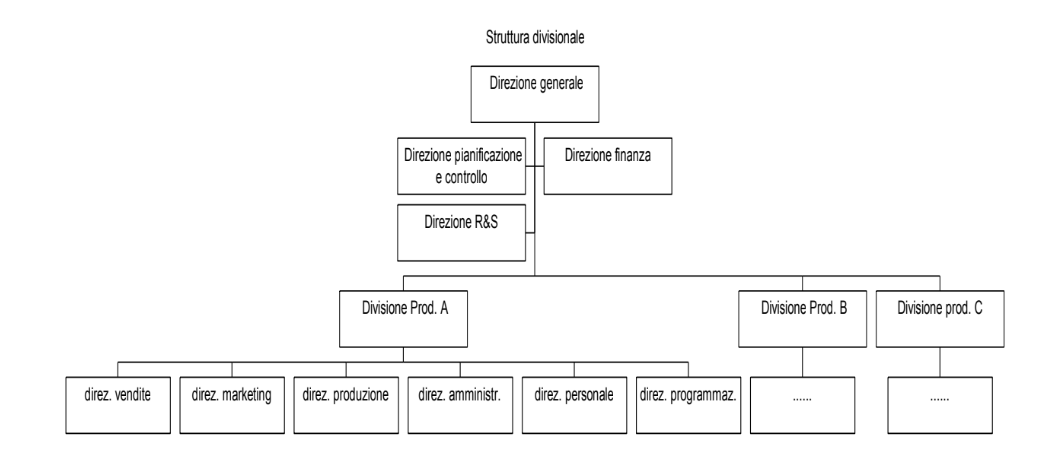
\includegraphics[scale = 0.50]{images/modello_divisionale.png}
    Esempio di modello divisionale
\end{center}

Un'azienda che adopera il modello divisionale è \textbf{Alphabet}, proprietaria
di Google.

\subsubsection{Il modello per Area Geografica}

Questo modello risulta simile al modello divisionale, con l'unica differenza che
le divisioni sono organizzate per area geografica. Questo tipo di struttura
aiuta l'azienda ad espandersi in nuovi mercati e a fare un uso più efficiente
delle risorse.

\begin{center}
    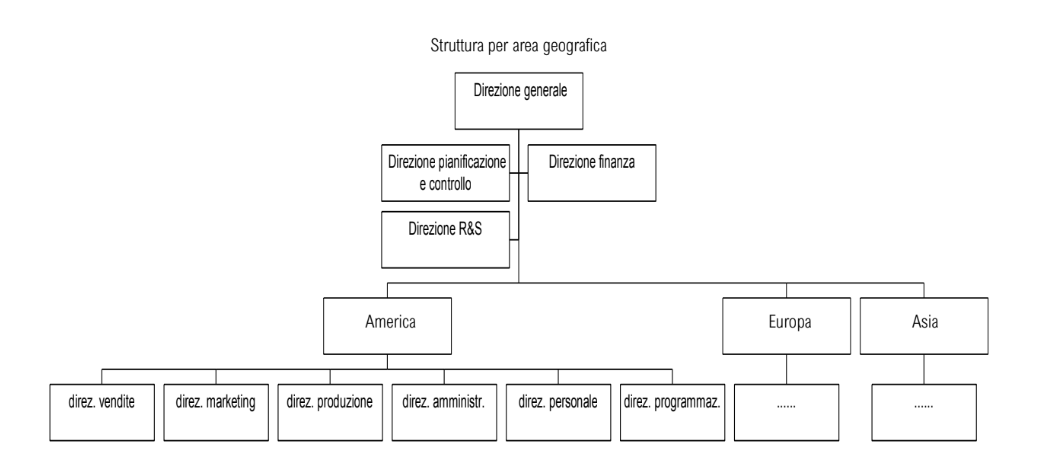
\includegraphics[scale=0.50]{images/modello_geografico.png}
    Esempio di modello per area geografica
\end{center}

\subsubsection{Il modello a Matrice}

Questo modello cerca di combinare al meglio i vantaggi dell' \\ 
organizzazione per funzioni con quelli dell'organizzazione per prodotti o
progetti.

\begin{center}
    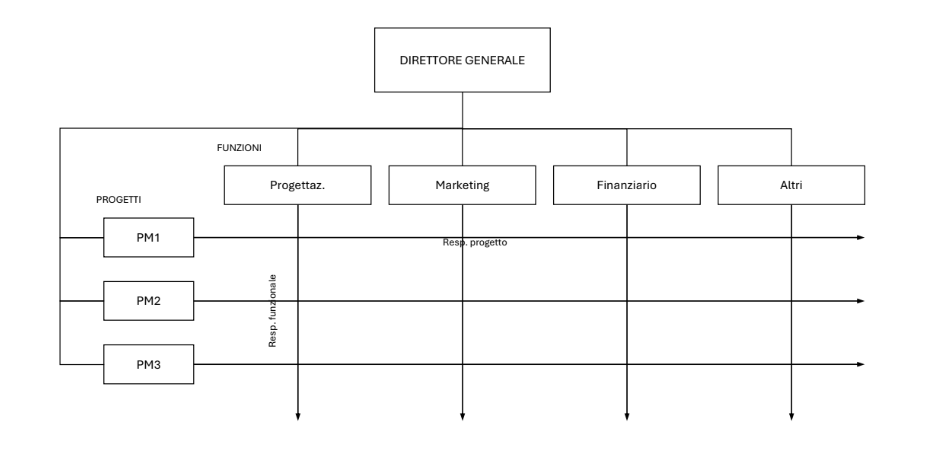
\includegraphics[scale=0.60]{images/modello_matrice.png}
    Esempio di modello a matrice
\end{center}
Molte aziende adoperano questo tipo di struttura, tra le più celebri troviamo
Intel, Spotify, Microsoft, IBM, Philips.

\subsubsection{Il modello a Rete}

Questo modello affida varie parti dell'organizzazione a partner esterni. In
questo caso si parla di \textbf{Outsourcing}, ovvero quando l'azienda ricorre a
fornitori esterni per determinati compiti o funzioni, quali la produzione, le
risorse umane o la gestione dei crediti.

\begin{center}
    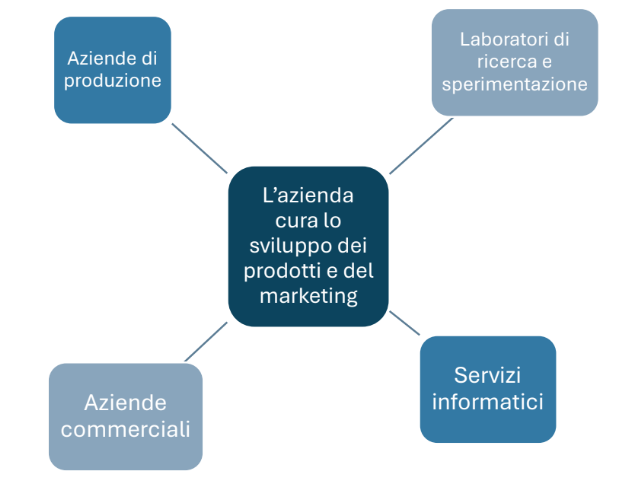
\includegraphics[scale=0.80]{images/modello_rete.png}
\end{center}
Un grande esempio di azienda che adopera questa struttura è Nike, che affida la
produzione e la distribuzione dei propri prodotti ad aziende esterne.

\section{Lezione 4}

\subsection{Stadi dello Sviluppo di un'azienda}

In questo capitolo andremo ad osservare i vari stadi dello sviluppo di
un'azienda, le varie crisi e le soluzioni che vengono adottate per poter
progredire.

\subsubsection{Stadio imprenditoriale}

Quando un'impresa è ancora allo stato embrionale, l'enfasi è posta sulla
\textbf{creazione} di un prodotto o un servizio e sulla \textbf{sopravvivenza}
nel mercato. L'organizzazione in questo momento risulta informale e non
burocratica, vi è un controllo diretto da parte del proprietario.

\begin{center}
    \textcolor{red!50}{Crisi: Bisogno di leadership}

    man mano che l'organizzazione cresce con l'aumento del numero dei dipendenti
    vengono a crearsi problemi relativi alla gestione, gli imprenditori si
    trovano costretti ad adattare una struttura organizzativa per assecondare un
    processo continuo di crescita.
\end{center}

\subsubsection{Stadio della collettività}

Se la crisi di leadership viene superata, si ottiene una direzione forte e
inizia lo sviluppo di obiettivi e di una direzione chiara dell'azienda. Vengono
strutturate le unità organizzative insieme ad una gerarchia di autorità, vengono
definiti i compiti e una prima divisione del lavoro. In questo stadio i
dipendenti cominciano ad \textbf{identificarsi} nella missione
dell'organizzazione ed idealmente dedicano molto tempo a contribuire al successo
organizzativo. La comunicazione e il controllo continuano ad essere
prevalentemente informali, comincia a nascere qualche sistema formale

\begin{center}
    \textcolor{red!50}{Crisi: Bisogno di delega}

    se il management ha operato con successo, i dipendenti a livelli inferiori
    si trovano limitati dalla forte leadership esercitata dall'alto, d'altra
    parte i manager di livello inferiore cominciano a chiedere una maggiore
    fiducia, l'organizzazione si trova dunque a dover escogitare un meccanismo
    per coordinare le diverse unità senza la supervisione del vertice.
\end{center}

\subsubsection{Stadio della formalizzazione}

Vengono introdotte nuove regole, procedure e sistemi di controllo. La
comunicazione diviene formale e segue la linea gerarchica. La direzione comincia
ad interessarsi maggiormente a strategia e pianificazione lasciando gli aspetti
produttivi ad un livello più basso di management.

\begin{center}
    \textcolor{red!50}{Crisi: Eccesso di burocrazia}

    Lo sviluppo dell'organizzazione porta ad una proliferazione di sistemi e
    procedure che possono cominciare a soffocare i manager dei livelli
    intermedi. L'organizzazione risulta troppo grande e complessa per essere
    gestita da programmi formali.
\end{center}

\subsubsection{Stadio di elaborazione}

La soluzione all'ultima crisi consiste nel far raggiungere alla burocrazia il
suo limite superiore (oltre il quale avremmo un eccesso), i manager imparano a
lavorare all'interno della burocrazia senza doverla accrescere. In questi casi
l'azienda può anche essere scomposta in divisioni per mantenere la filosofia da
piccola azienda.

\begin{center}
    \textcolor{red!50}{Crisi: Bisogno di rivitalizzazione}

    Dopo che l'azienda ha raggiunto la maturità è possibile che si cominci a
    manifestare un bisogno di rinnovamento, che può essere sentito con cadenze
    che vanno dai 10 ai 20 anni. L'azienda si disallinea rispetto all'ambiente
    in cui opera o diventa lenta e troppo burocratica, deve passare attraverso
    uno stadio di snellimento e innovazione.
\end{center}

\begin{center}
    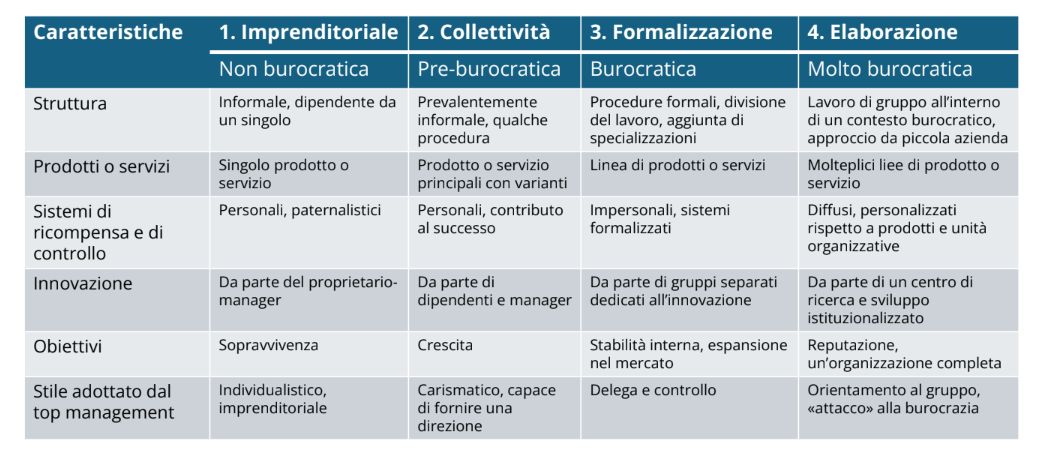
\includegraphics[scale=0.50]{images/stati_sviluppo.png}
    Mappa degli stadi di sviluppo
\end{center}

\subsection{Stadi del Declino di un'azienda}

Sulla base di un ampio studio sul declino organizzativo è stato \\
proposto un modello che attraversa 5 stadi fino alla \textbf{dissoluzione}
dell'organizzazione.

\subsubsection{Stadio della cecità}

Essendo il primo stadio, risulta complesso per il management avvertire i segnali
di declino, che possono presentarsi sotto forma di:

\begin{enumerate}
    \item Personale in eccesso;
    \item Procedure troppo complesse;
    \item Mancanza di allineamento con il proprio target;
    \item Ecc. 
\end{enumerate}
La soluzione per prevenire questo stato di \textbf{cecità} è mettere \\ in campo
sistemi di monitoraggio e di controllo che indichino prontamente quando qualcosa
non funziona, infatti potendo contare su informazioni tempestive il management
può riportare l'organizzazione alle prestazioni ottimali.

\subsubsection{Stadio dell'inattività}

Questo stadio deriva da una mancata attenzione alle condizioni correnti di
declino malgrado eventuali segni di calo delle prestazioni. La soluzione per
prevenire l'\textbf{inattività} è riconoscere l'eventuale declino e
intraprendere azioni rapide per riallineare l'organizzazione. Queste azioni
possono comprendere:

\begin{enumerate}
    \item Nuovi approcci alla risoluzione dei problemi;
    \item Maggiore partecipazione al processo decisionale;
    \item Incoraggiamento delle manifestazioni di insoddisfazione da parte dei
    dipendenti e dei clienti per capire cosa non funziona.   
\end{enumerate}

\subsubsection{Stadio dell'errore}

In questo stadio l'organizzazione affronta i problemi gravi e gli indicatori che
mostrano che i cattivi risultati non possono più essere ignorati. Il management
è quindi costretto a ricorrere a cambiamenti drastici.

Le possibilità per far fronte a questa situazione possono essere:

\begin{enumerate}
    \item Ridurre i costi, tagliando il personale;
    \item Ridurre l'incertezza dei dipendenti chiarendo valori e fornendo
    informazioni;  
\end{enumerate}

Un errore commesso in questo stadio può sancire il \textbf{punto di non ritorno}
per l'organizzazione.

\subsubsection{Stadio della crisi}

A questo punto non si è stati ancora in grado di gestire in modo efficace il
declino e ci si trova in una situazione di panico. L'unica soluzione è una
\textbf{radicale riorganizzazione}. Vengono intraprese soluzioni drastiche, come
la sostituzione del management, rivoluzioni a livello di struttura, strategia e
cultura. In questo caso il taglio della forza lavoro può essere molto severo.

\subsubsection{Stadio della dissoluzione}

Questo stadio risulta irreversibile. L'organizzazione subisce perdite ingenti di
quote di mercato e di reputazione, dei suoi migliori talenti e dei capitali.
L'unica azione possibile è quella di porre fine all'organizzazione in maniera
ordinata.

\begin{center}
    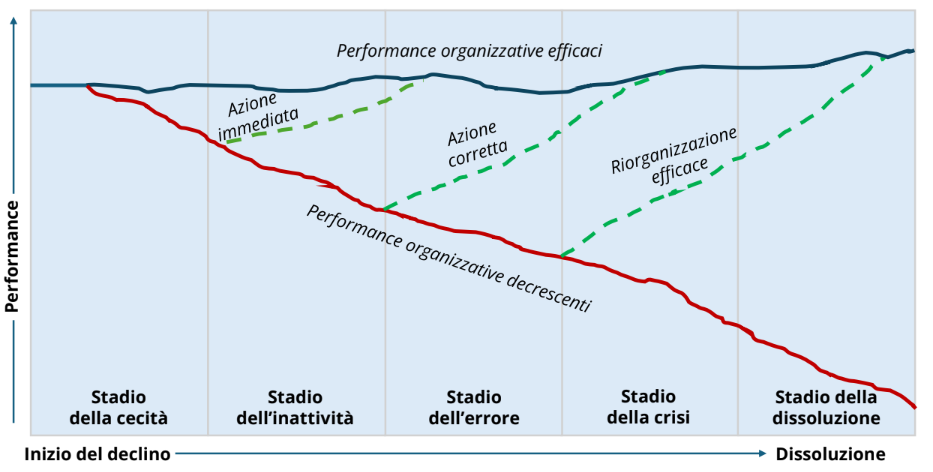
\includegraphics[scale=0.60]{images/stadi_declino.png}
    Mappa degli stadi del declino
\end{center}

\newpage
\subsection{I diversi tipi di Azienda in Italia}



\end{document}